\documentclass{article}
\usepackage{amsmath}
\usepackage{graphicx} % Required for inserting images
\usepackage{float}    % For placing images
\usepackage{subfigure} % For side-by-side images
\usepackage{hyperref}

\title{Experiment 6-Band Pass Sallen-Key Filter}
\author{Arnav Yadnopavit - EE24BTECH11007 \\ Prajwal - EE24BTECH11051}

\begin{document}

\maketitle

\section{Objective}
\begin{enumerate}
    \item To design and implement a bandpass filter using separate Sallen-Key Low Pass Filter (LPF) and High Pass Filter (HPF).
    \item To analyze and compare the frequency response of LPF, HPF, and the final bandpass filter.
    \item To plot the magnitude response (gain vs. frequency) of all three filters.
\end{enumerate}

\section{Theory}
A bandpass filter (BPF) allows only the frequencies within a specific range and does not allow outside it.
\begin{itemize}
    \item A High Pass Filter (HPF) to remove low-frequency components.
    \item A Low Pass Filter (LPF) to remove high-frequency components.
    \item The combined response results in a bandpass characteristic.
\end{itemize}

\subsection{Sallen-Key Second-Order Filters:}
\begin{itemize}
    \item It is an active filter topology using operational amplifiers.
    \item Provides a Butterworth, Bessel, or Chebyshev response based on component selection.
    \item The transfer function is given by:
    \begin{align}
        H(s)=\frac{s^2}{s^2+(\omega_c/Q)s+\omega_c^2}
    \end{align}
    where:\\
    $\omega_c$ is the cutoff frequency
    \begin{align}
        \omega_c=\frac{1}{\sqrt{R_1R_2C_1C_2}}
    \end{align}
    $Q$ is the quality factor
    \begin{align}
        Q=\frac{\sqrt{R_1R_2C_1C_2}}{C_2(R_1+R_2)}
    \end{align}
\end{itemize}

\subsection{Components and Equipment Required:}
\begin{itemize}
    \item Operational Amplifiers (e.g., TL074, TL081, or LM358)
    \item Resistors: R$_1$, R$_2$, R$_3$, R$_4$ (in k$\Omega$)
    \item Capacitors: C$_1$,C$_2$, C$_3$, C$_4$ (in nF)
    \item Function Generator
    \item Oscilloscope or Spectrum Analyzer
    \item DC Power Supply (±12V)
    \item Breadboard and connecting wires
\end{itemize}

\section{Circuit design:}
\subsection{High pass Sallen-Key filter design:}

% Two images side by side
\begin{figure}[H]
    \centering
    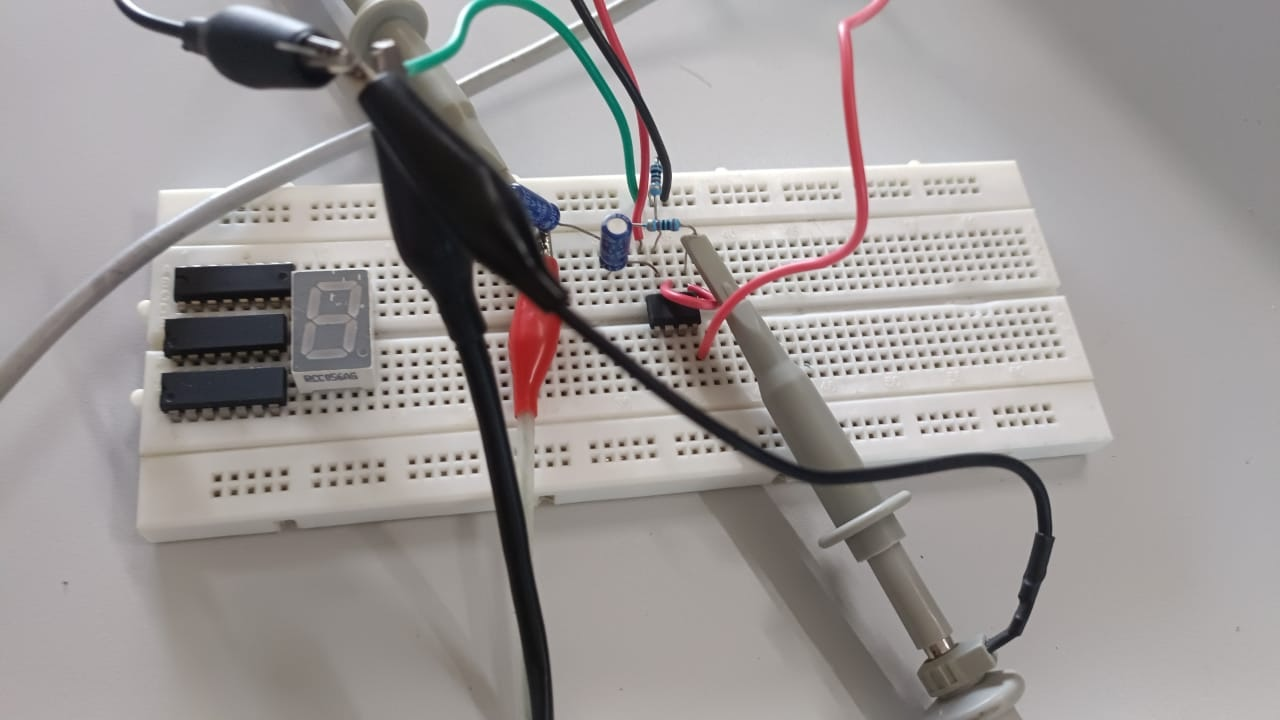
\includegraphics[width=0.8\textwidth]{figs/highpasscircuit.jpeg}
    \caption{High Pass Sallen-Key Filter-Circuit design}
\end{figure}

\begin{itemize}
    \item Here R$_1$=R$_2$=1000$\Omega$ and C$_1$=C$_2$=1$\mu$F
    \item Cutoff frequency $f_{c_1}$ (also lower cutoff frequency of the bandpass filter)
    \item Standard Sallen-Key HPF formula:
    \begin{align}
        f_c = \frac{1}{2\pi\sqrt{R_1R_2C_1C_2}}
    \end{align}
    Substituting values:
    \begin{align}
        f_c = \frac{1}{2\pi\sqrt{(1000)(1000)(1 \times 10^{-6})(1 \times 10^{-6})}}
    \end{align}
    \begin{align}
        f_c = 159.15 \text{ Hz}
    \end{align}
    \item Angular cutoff frequency:
    \begin{align}
        \omega_c = 2\pi f_c = 2\pi \times 159.15 = 1000 \text{ rad/sec}
    \end{align}
    \item Quality factor:
    \begin{align}
        Q = \frac{1}{2} = 0.5
    \end{align}
    \item Transfer function of the High Pass Filter:
    \begin{align}
        H(s) = \frac{s^2}{s^2 + \frac{\omega_c}{Q}s + \omega_c^2}
    \end{align}
    where:\\
    $s$ is the complex frequency variable, $s = j\omega$ \\
    $\omega_c = 1000$ rad/sec \\
    $Q = 0.5$
\end{itemize}

\textbf{Experimental Data}
\begin{table}[H]
    \centering
    \begin{tabular}{|c|c|c|c|c|}
        \hline
        Frequency (Hz) & Input Voltage (V) & Output Voltage (V) & Experimental Gain & Theoretical Gain\\
        \hline
        100 & 1.0 & 0.24 & -10.46 & -10.96 \\
        160 & 1.0 & 0.44 & -7.12 & -6.2 \\
        200 & 1.0 & 0.56 & -5.04 & -4.26 \\
        1000 & 1.0 & 0.76 & -0.238. & -0.217 \\
        \hline
    \end{tabular}
    \caption{Comparison of Experimental and Theoretical Gain for High Pass Filter}
    \label{tab:exp_data}
\end{table}
\begin{figure}[H]
    \centering
    \subfigure[Input]{
        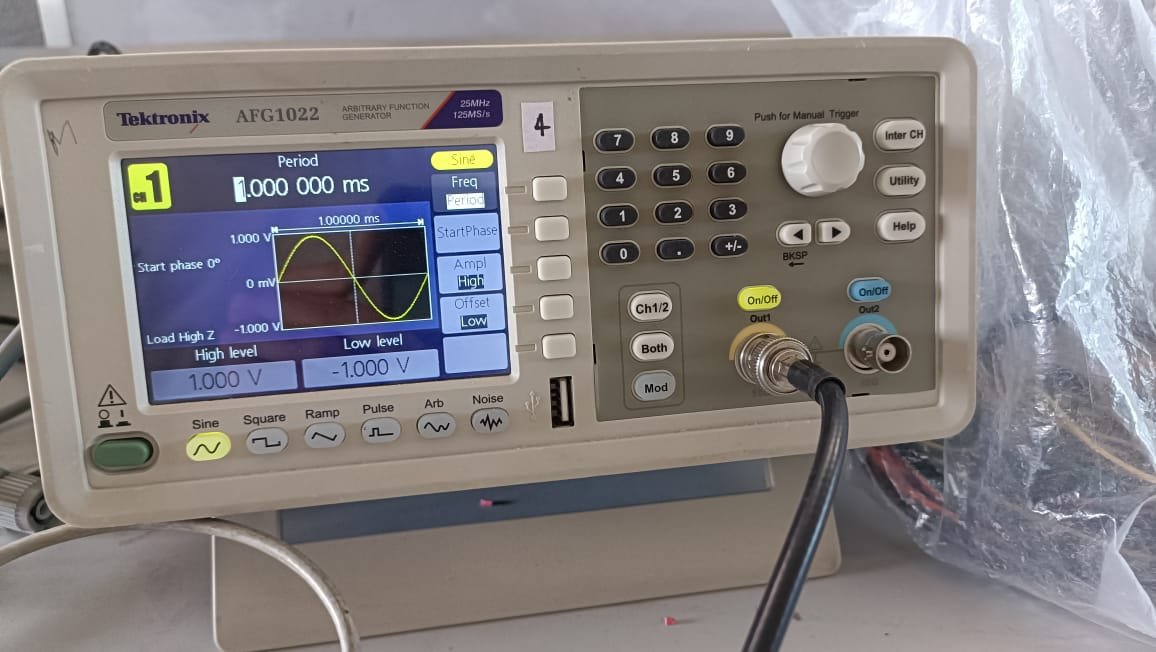
\includegraphics[width=0.45\textwidth]{figs/highpassin1.jpeg}
    }
    \hfill
    \subfigure[Output]{
        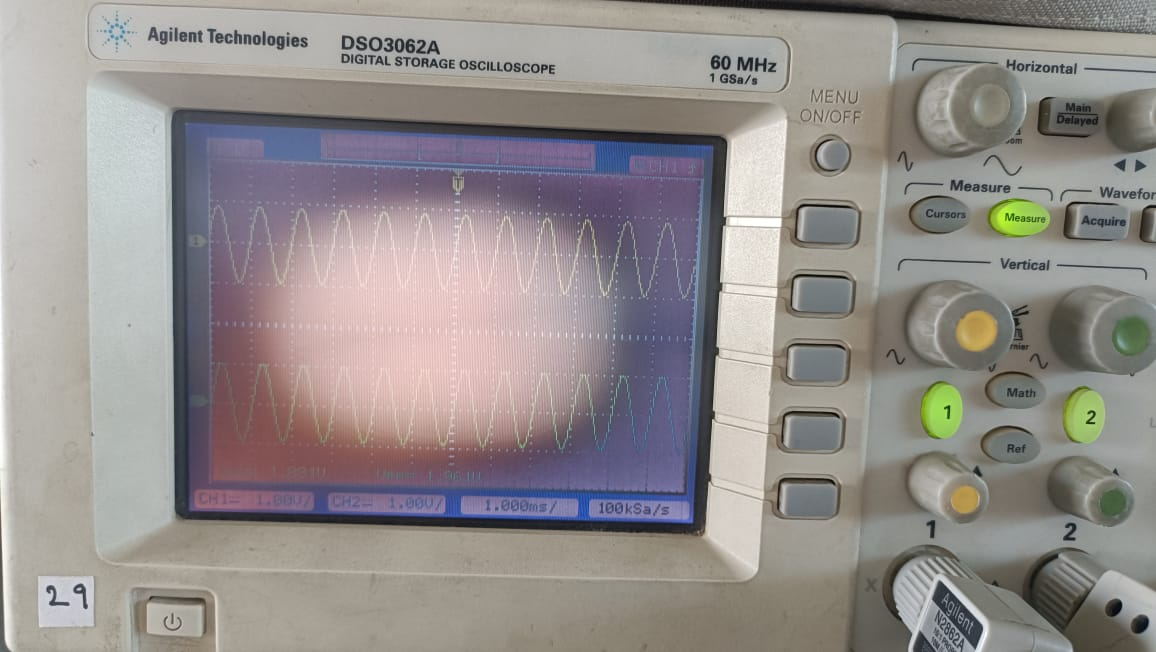
\includegraphics[width=0.45\textwidth]{figs/highpassout1.jpeg}
    }
\end{figure}
\begin{figure}[H]
    \centering
    \subfigure[Input]{
        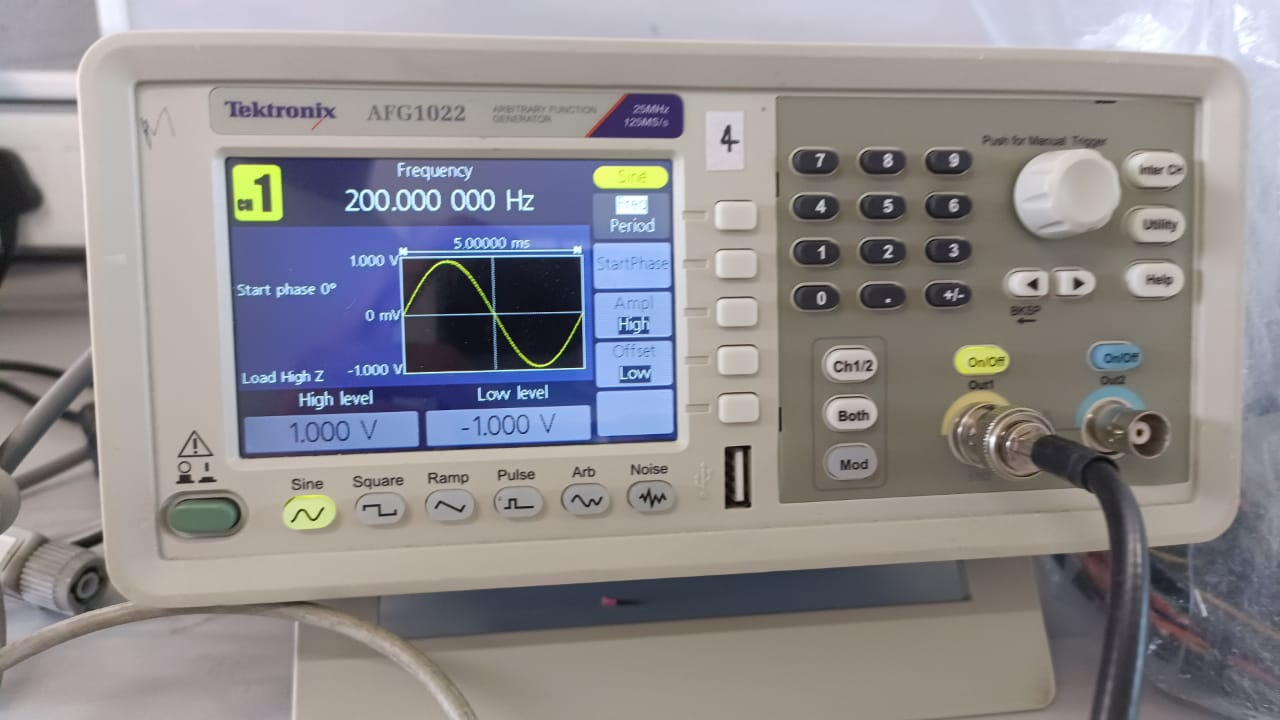
\includegraphics[width=0.45\textwidth]{figs/highpassin2.jpeg}
    }
    \hfill
    \subfigure[Output]{
        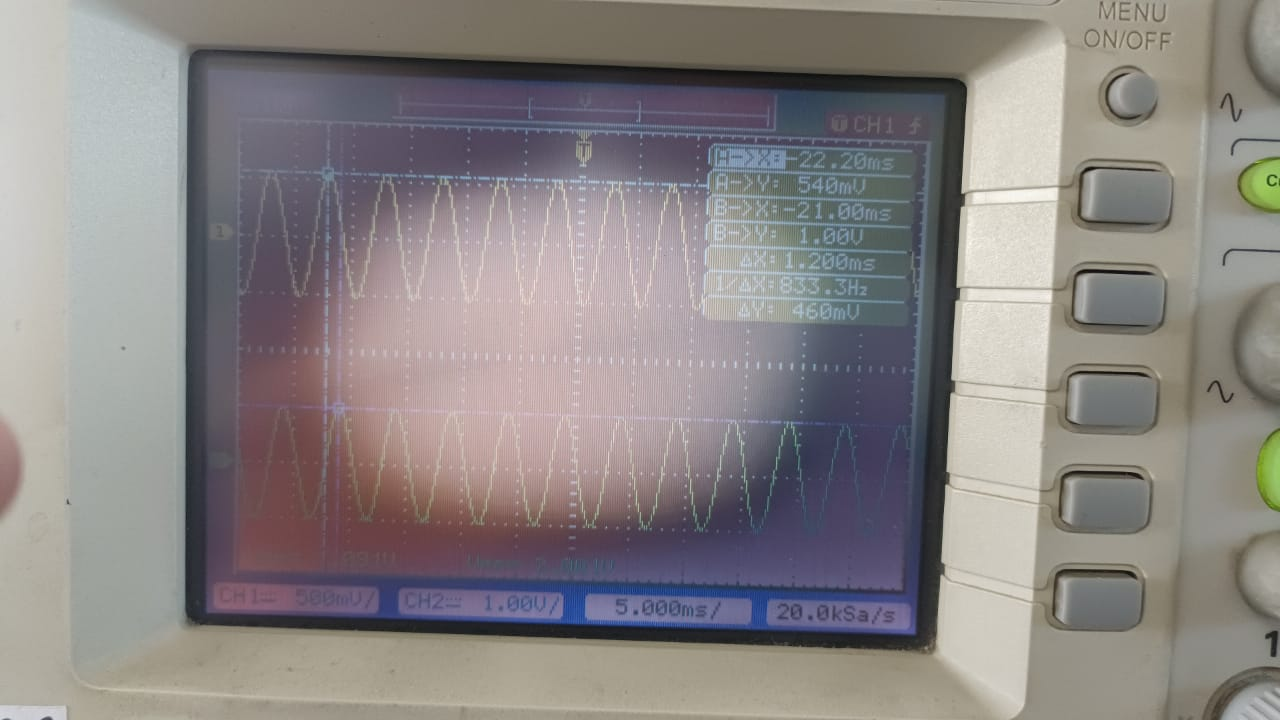
\includegraphics[width=0.45\textwidth]{figs/highpassout2.jpeg}
    }
\end{figure}
\begin{figure}[H]
    \centering
    \subfigure[Input]{
        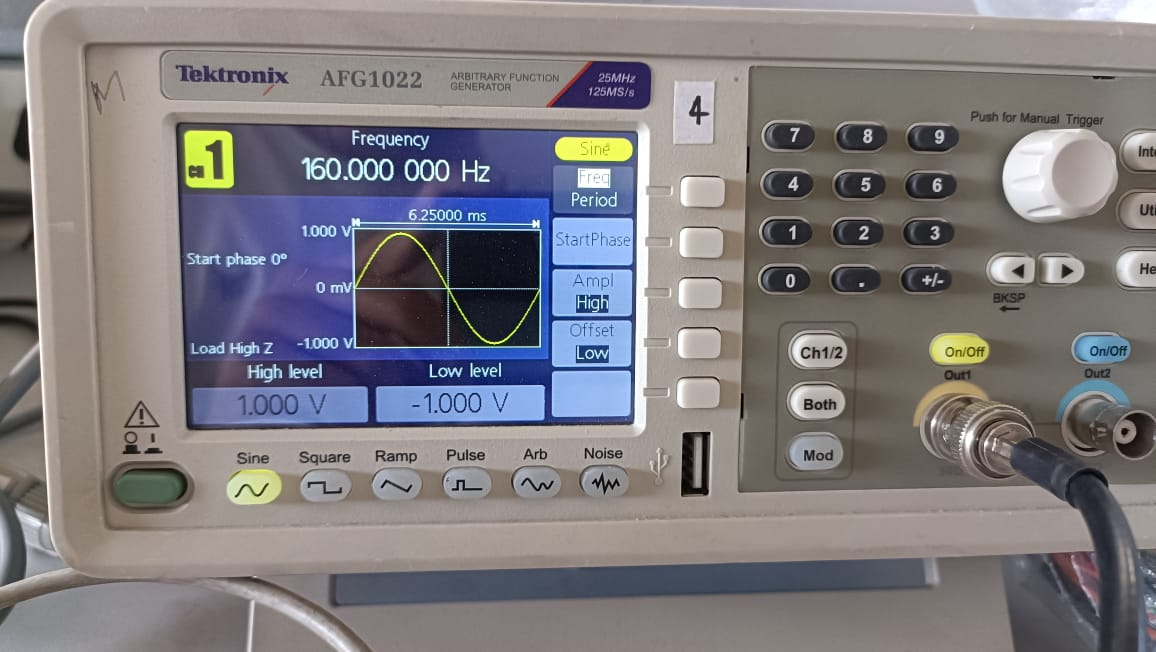
\includegraphics[width=0.45\textwidth]{figs/highpassin3.jpeg}
    }
    \hfill
    \subfigure[Output]{
        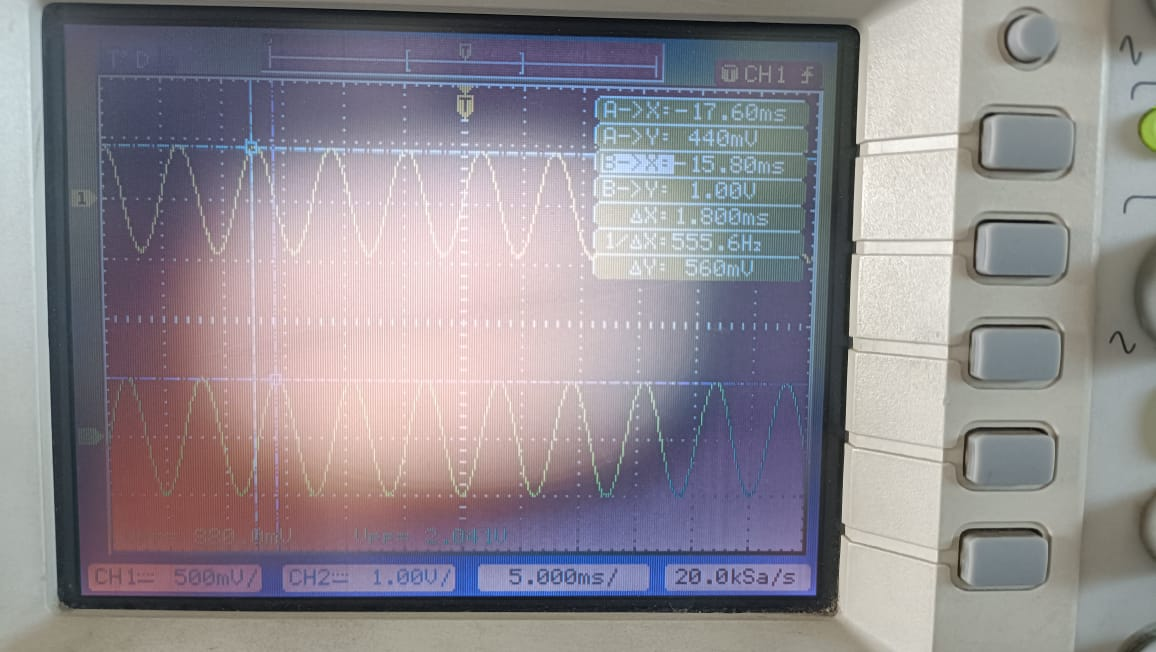
\includegraphics[width=0.45\textwidth]{figs/highpassout3.jpeg}
    }
\end{figure}
\begin{figure}[H]
    \centering
    \subfigure[Input]{
        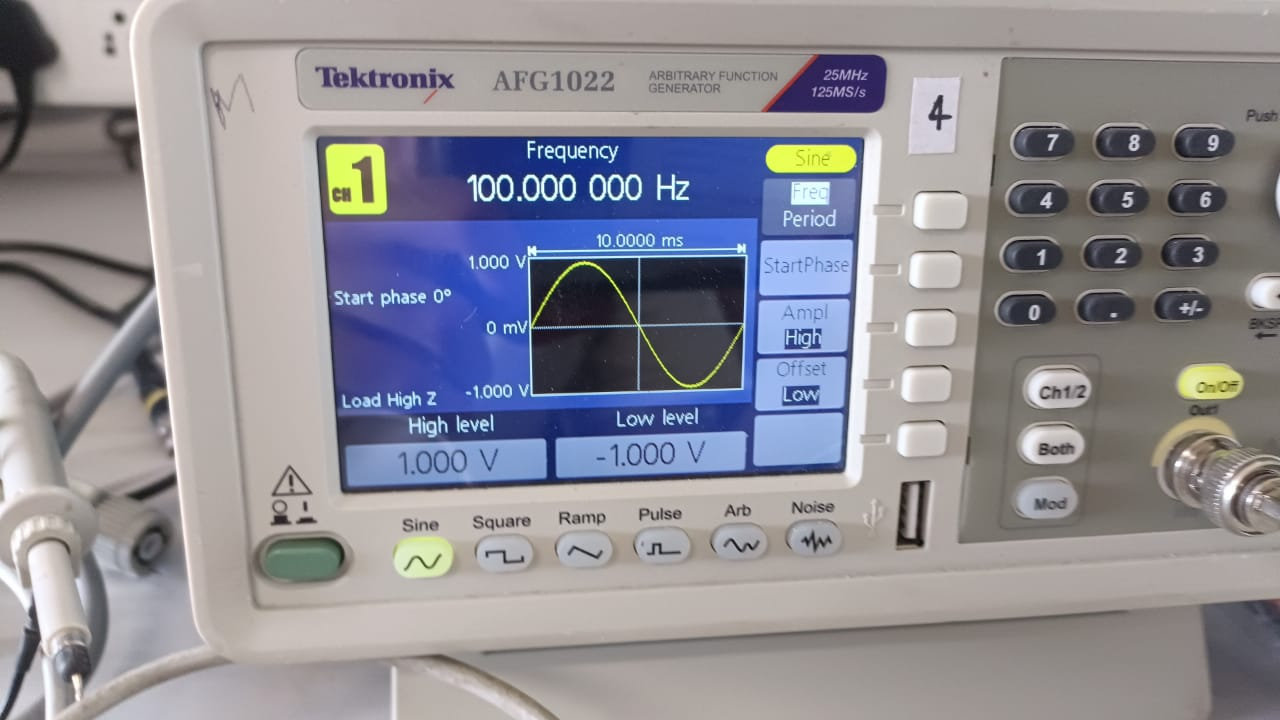
\includegraphics[width=0.45\textwidth]{figs/highpassin4.jpeg}
    }
    \hfill
    \subfigure[Output]{
        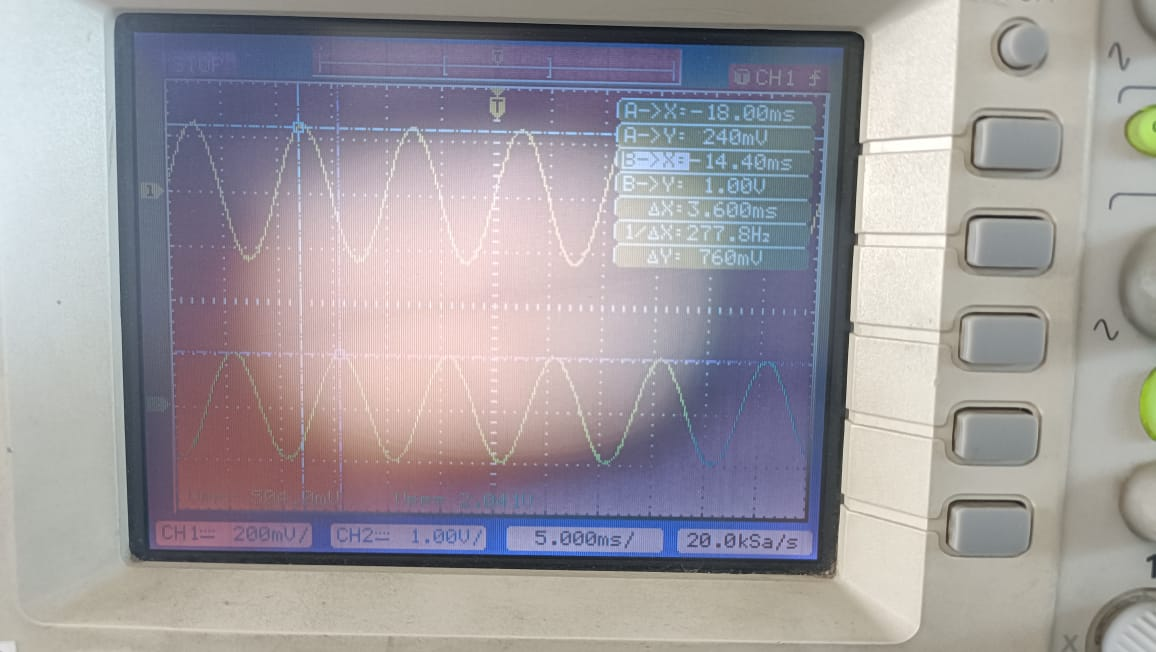
\includegraphics[width=0.45\textwidth]{figs/highpassout4.jpeg}
    }
    \caption{Experimental results for high pass filter}
\end{figure}

% Add highpass.png at the end of the high-pass filter section
\begin{figure}[H]
    \centering
    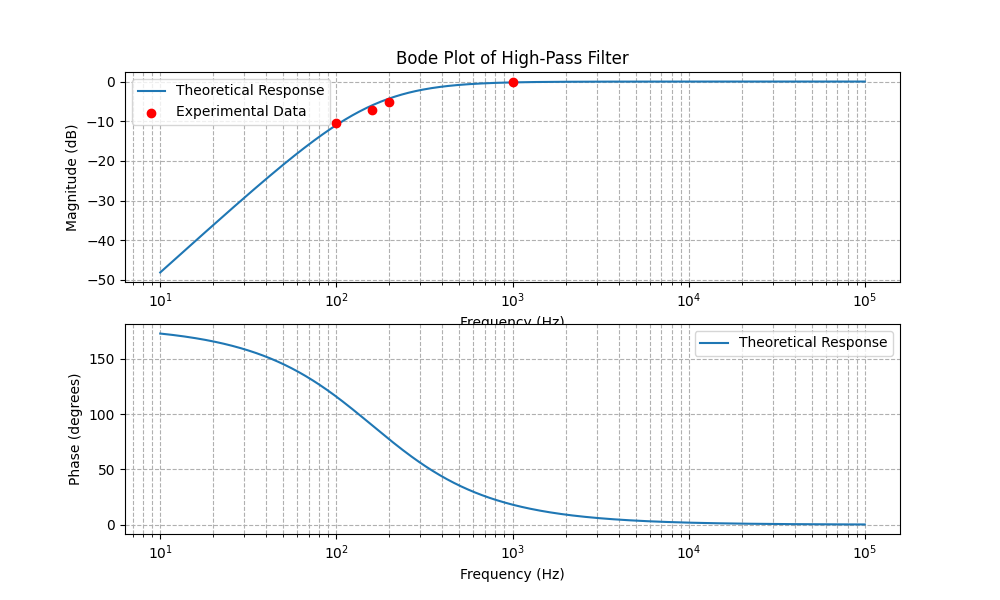
\includegraphics[width=0.8\textwidth]{figs/highpass.png}
    \caption{High Pass Filter Frequency Response}
\end{figure}

\subsection{Low pass Sallen-Key filter design:}

% Two images side by side
\begin{figure}[H]
    \centering
    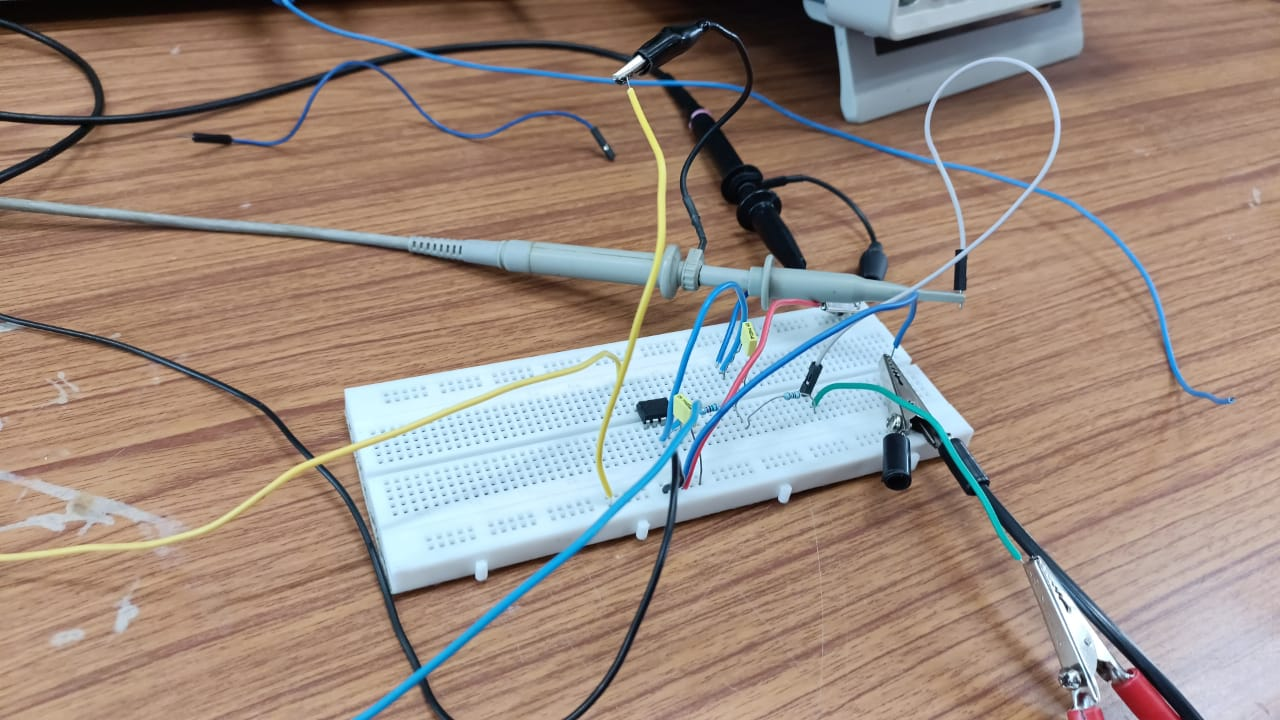
\includegraphics[width=0.8\textwidth]{figs/lowpasscircuit.jpeg}
    \caption{Low Pass Sallen-Key Filter-Circuit design}
\end{figure}

\begin{itemize}
    \item Here R$_1$=R$_2$=1000$\Omega$ and C$_1$=C$_2$=1$\mu$F
    \item Cutoff frequency $f_{c_2}$ (also upper cutoff frequency of the bandpass filter)
    \item Standard Sallen-Key LPF formula:
    \begin{align}
        f_c = \frac{1}{2\pi\sqrt{R_1R_2C_1C_2}}
    \end{align}
    Substituting values:
    \begin{align}
        f_c = \frac{1}{2\pi\sqrt{(1000)(1000)(1 \times 10^{-6})(1 \times 10^{-6})}}
    \end{align}
    \begin{align}
        f_c = 159.15 \text{ Hz}
    \end{align}
    \item Angular cutoff frequency:
    \begin{align}
        \omega_c = 2\pi f_c = 2\pi \times 159.15 = 1000 \text{ rad/sec}
    \end{align}
    \item Quality factor:
    \begin{align}
        Q = \frac{1}{2} = 0.5
    \end{align}
    \item Transfer function of the Low Pass Filter:
    \begin{align}
        H(s) = \frac{\omega_c^2}{s^2 + \frac{\omega_c}{Q}s + \omega_c^2}
    \end{align}
    where:\\
    $s$ is the complex frequency variable, $s = j\omega$ \\
    $\omega_c = 1000$ rad/sec \\
    $Q = 0.5$
\end{itemize}

\textbf{Experimental Data}
\begin{table}[H]
    \centering
    \begin{tabular}{|c|c|c|c|c|}
        \hline
        Frequency (Hz) & Input Voltage (V) & Output Voltage (V) & Experimental Gain & Theoretical Gain\\
        \hline
        100 & 1.8 & 1.62 & -2.38 & -2.88 \\
        160 & 1.0 & 0.88 & -5.36 & -6.08 \\
        500 & 1.0 & 0.124 & -18.12 & -20.72 \\
        1000 & 1.0 & 0.48 & -28.2 & -31.5 \\
        \hline
    \end{tabular}
    \caption{Comparison of Experimental and Theoretical Gain for Low Pass Filter}
    \label{tab:exp_data_lpf}
\end{table}
\begin{figure}[H]
    \centering
    \subfigure[Input]{
        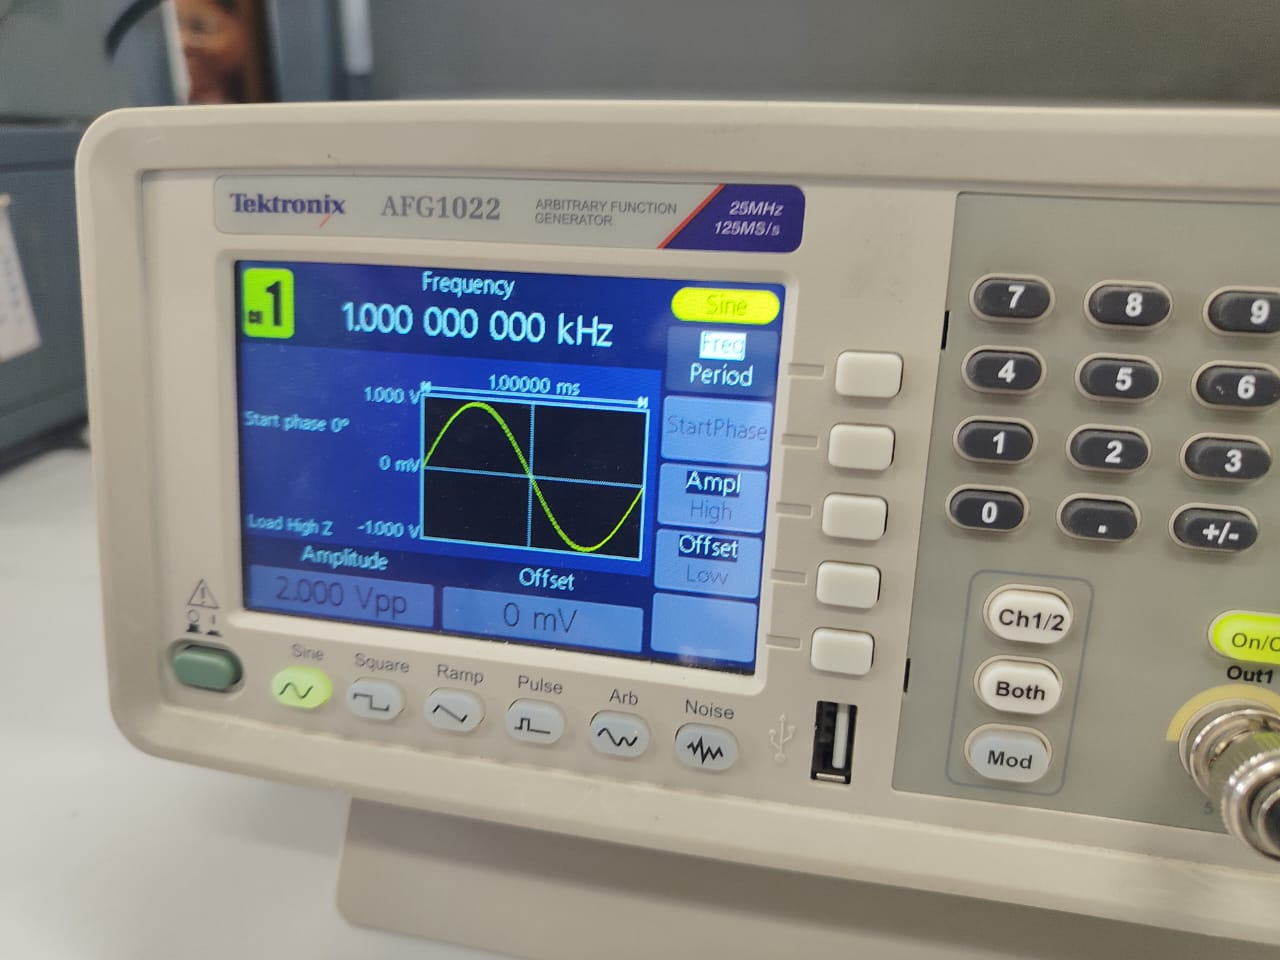
\includegraphics[width=0.45\textwidth]{figs/lowpassin1.jpeg}
    }
    \hfill
    \subfigure[Output]{
        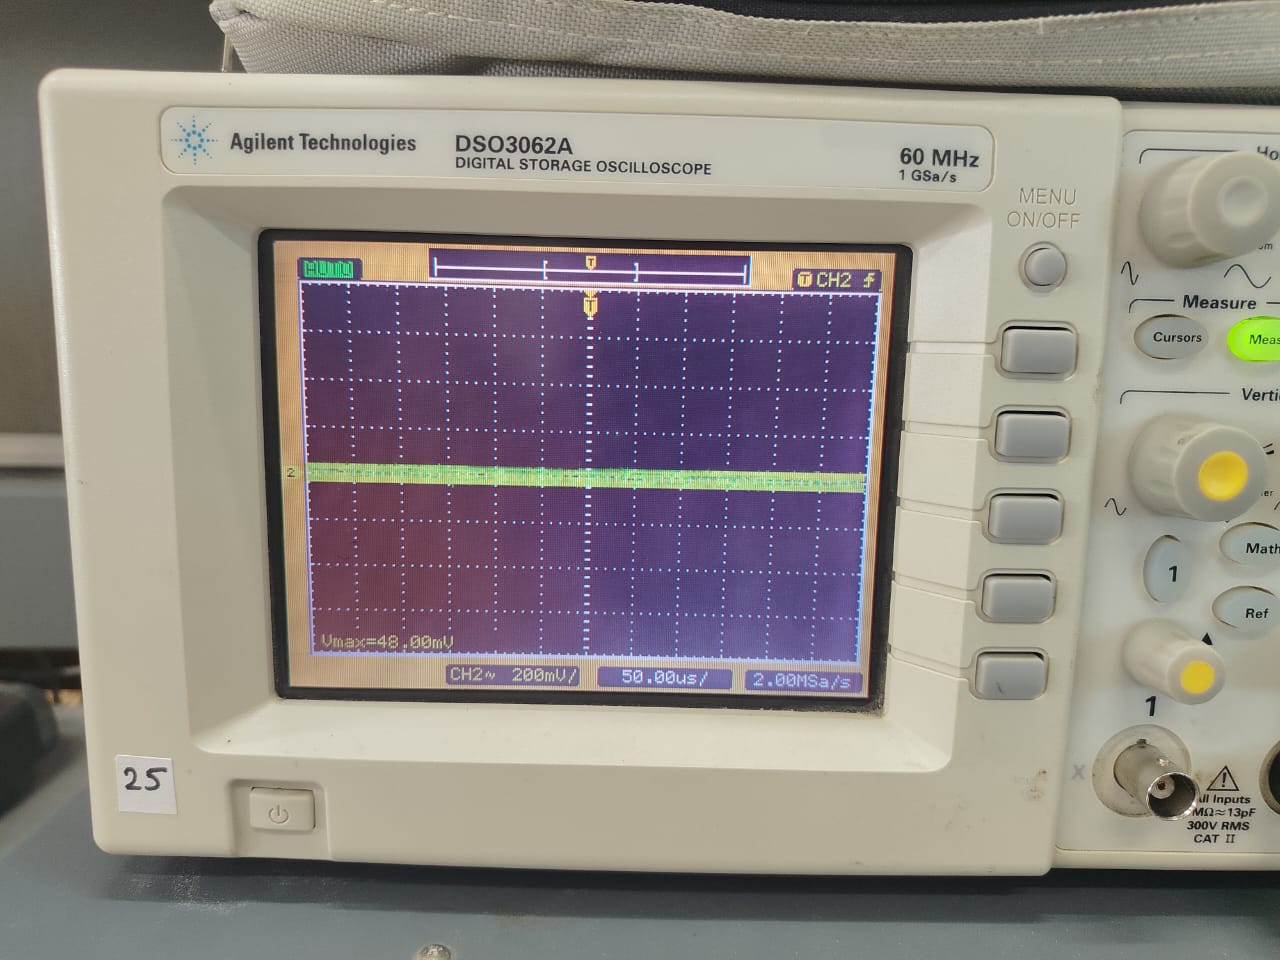
\includegraphics[width=0.45\textwidth]{figs/lowpassout1.jpeg}
    }
\end{figure}
\begin{figure}[H]
    \centering
    \subfigure[Input]{
        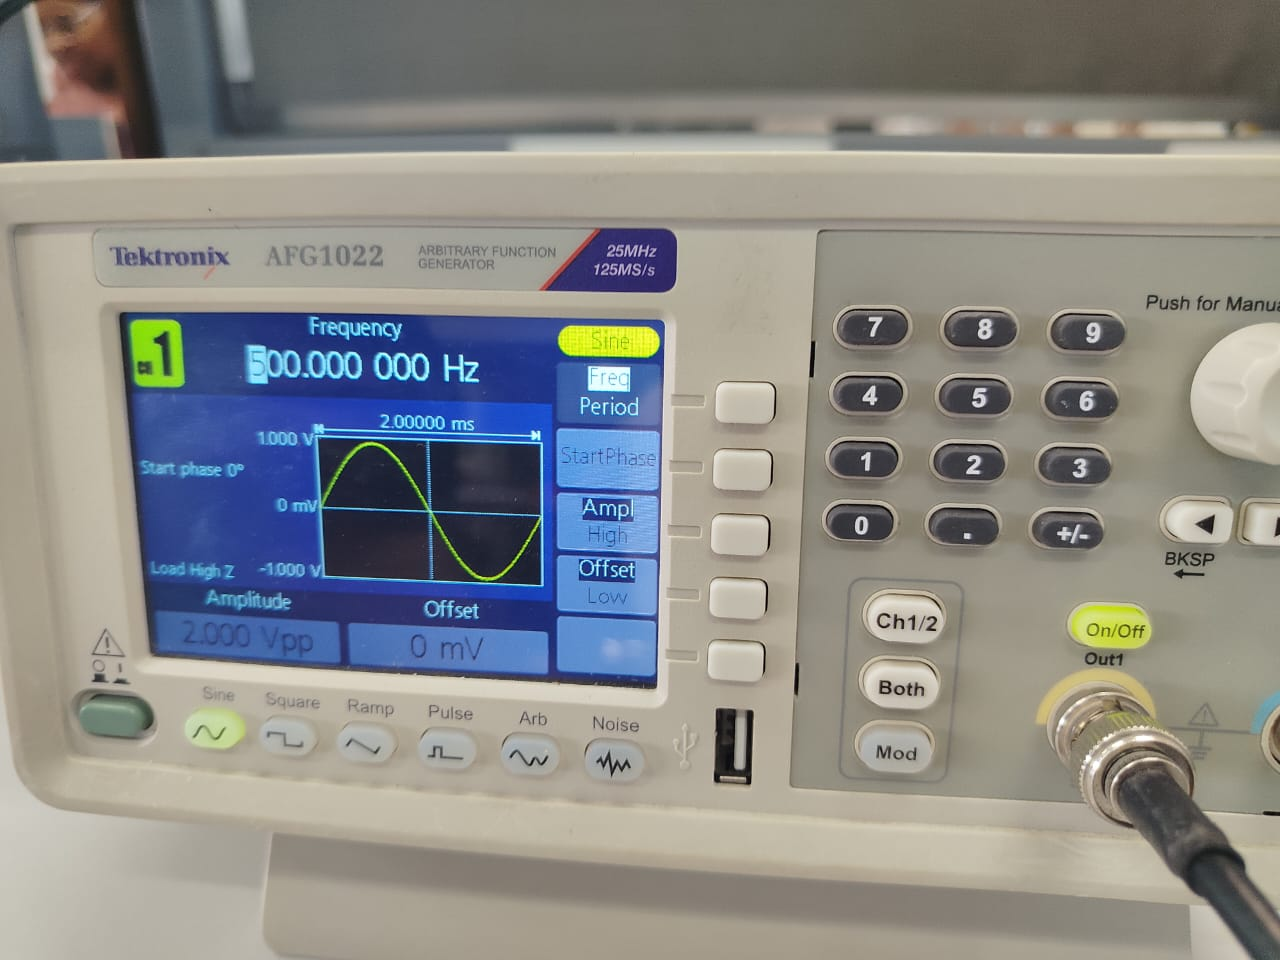
\includegraphics[width=0.45\textwidth]{figs/lowpassin2.jpeg}
    }
    \hfill
    \subfigure[Output]{
        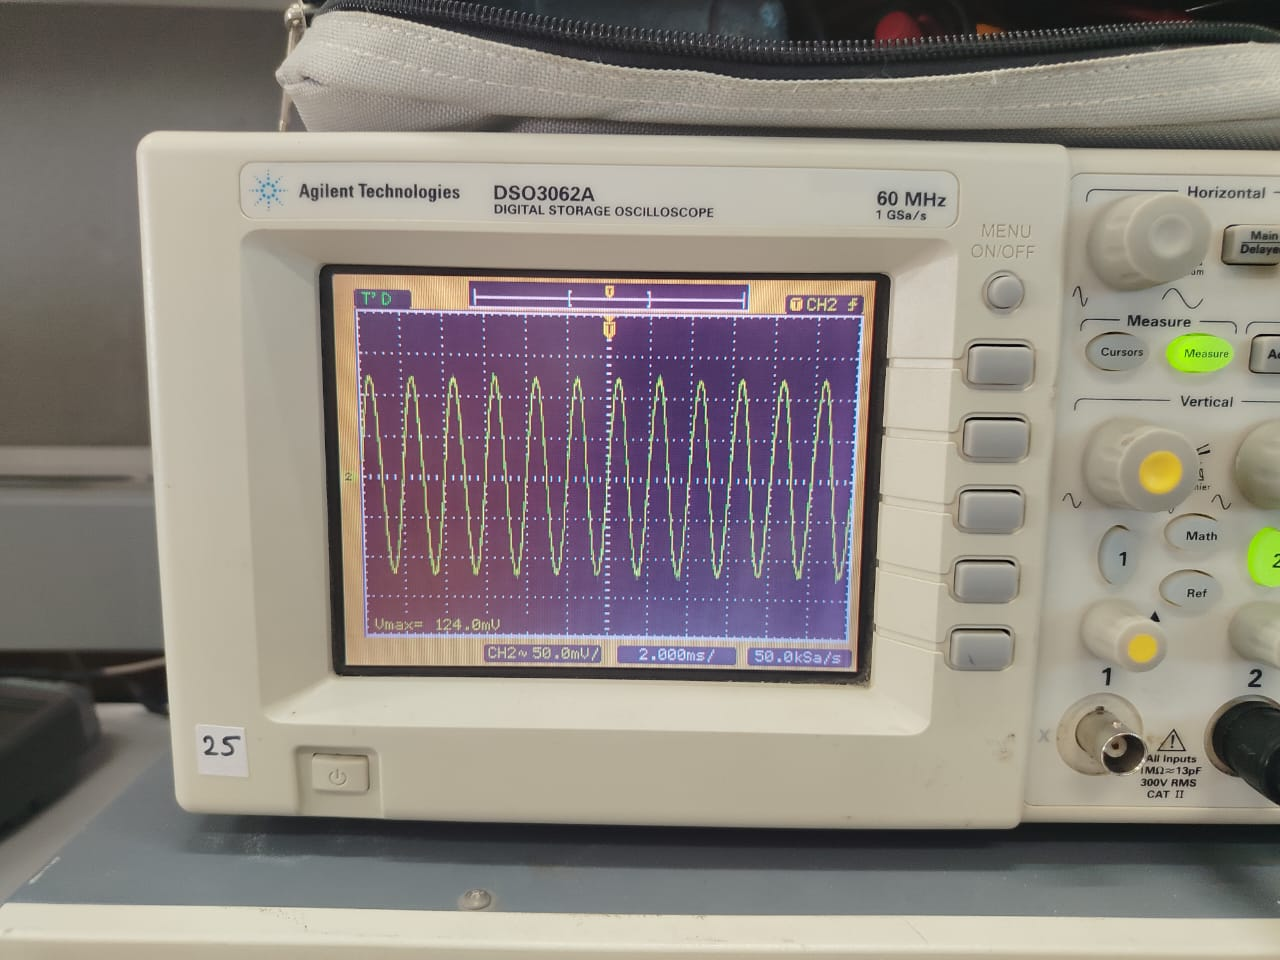
\includegraphics[width=0.45\textwidth]{figs/lowpassout2.jpeg}
    }
\end{figure}
\begin{figure}[H]
    \centering
    \subfigure[Input]{
        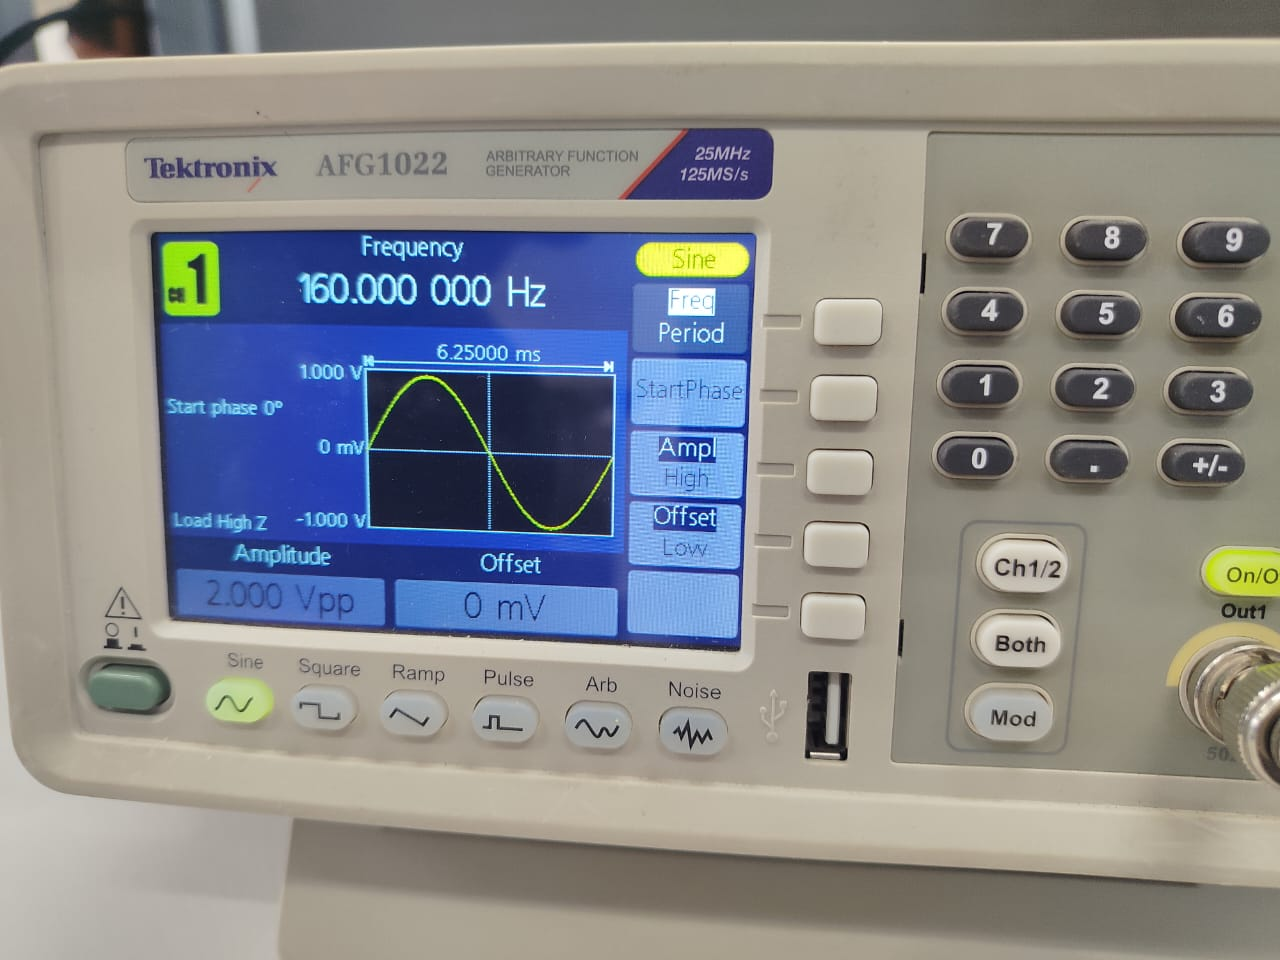
\includegraphics[width=0.45\textwidth]{figs/lowpassin3.jpeg}
    }
    \hfill
    \subfigure[Output]{
        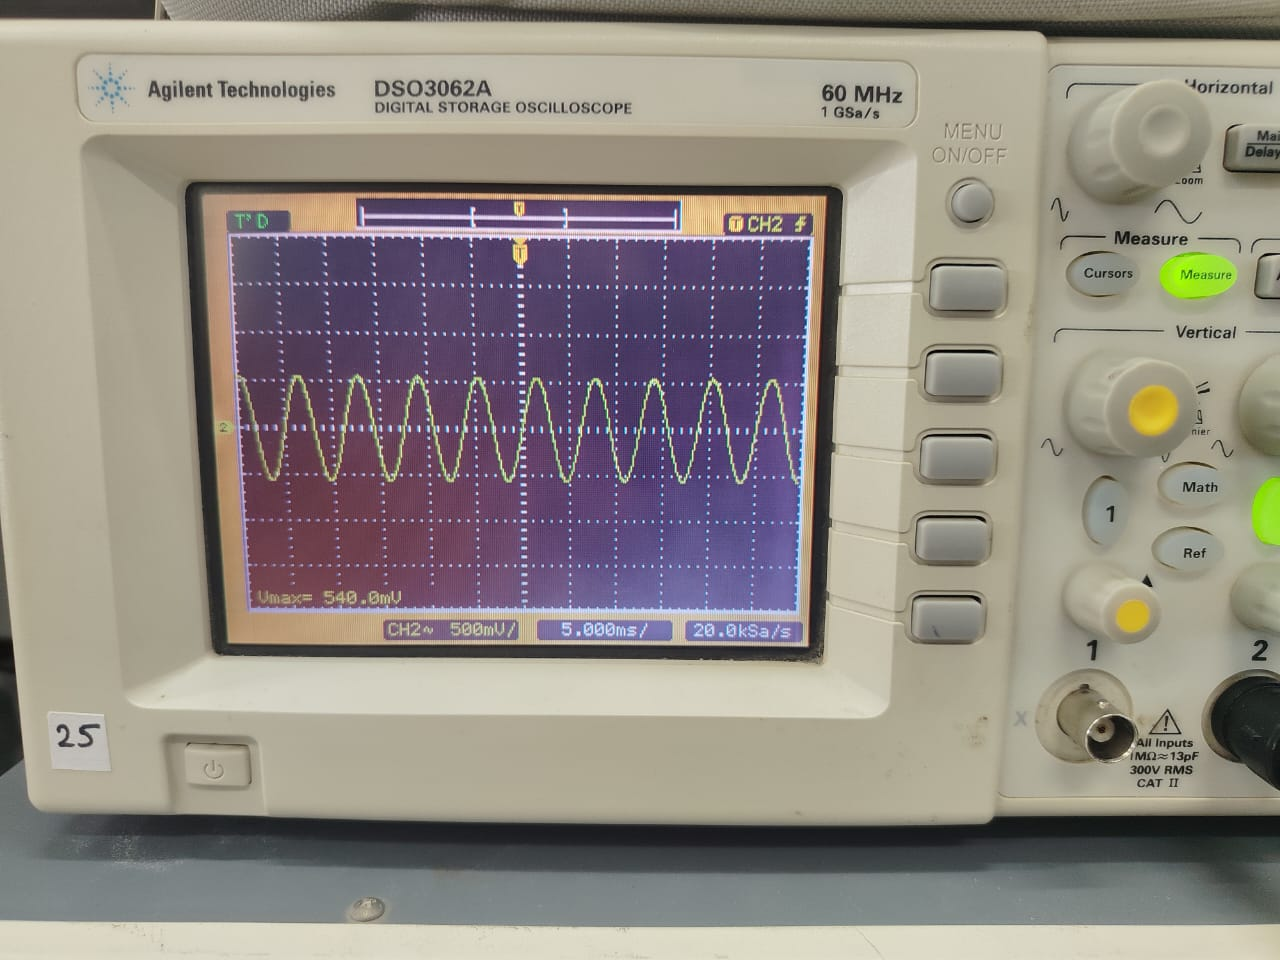
\includegraphics[width=0.45\textwidth]{figs/lowpassout3.jpeg}
    }
\end{figure}
\begin{figure}[H]
    \centering
    \subfigure[Input]{
        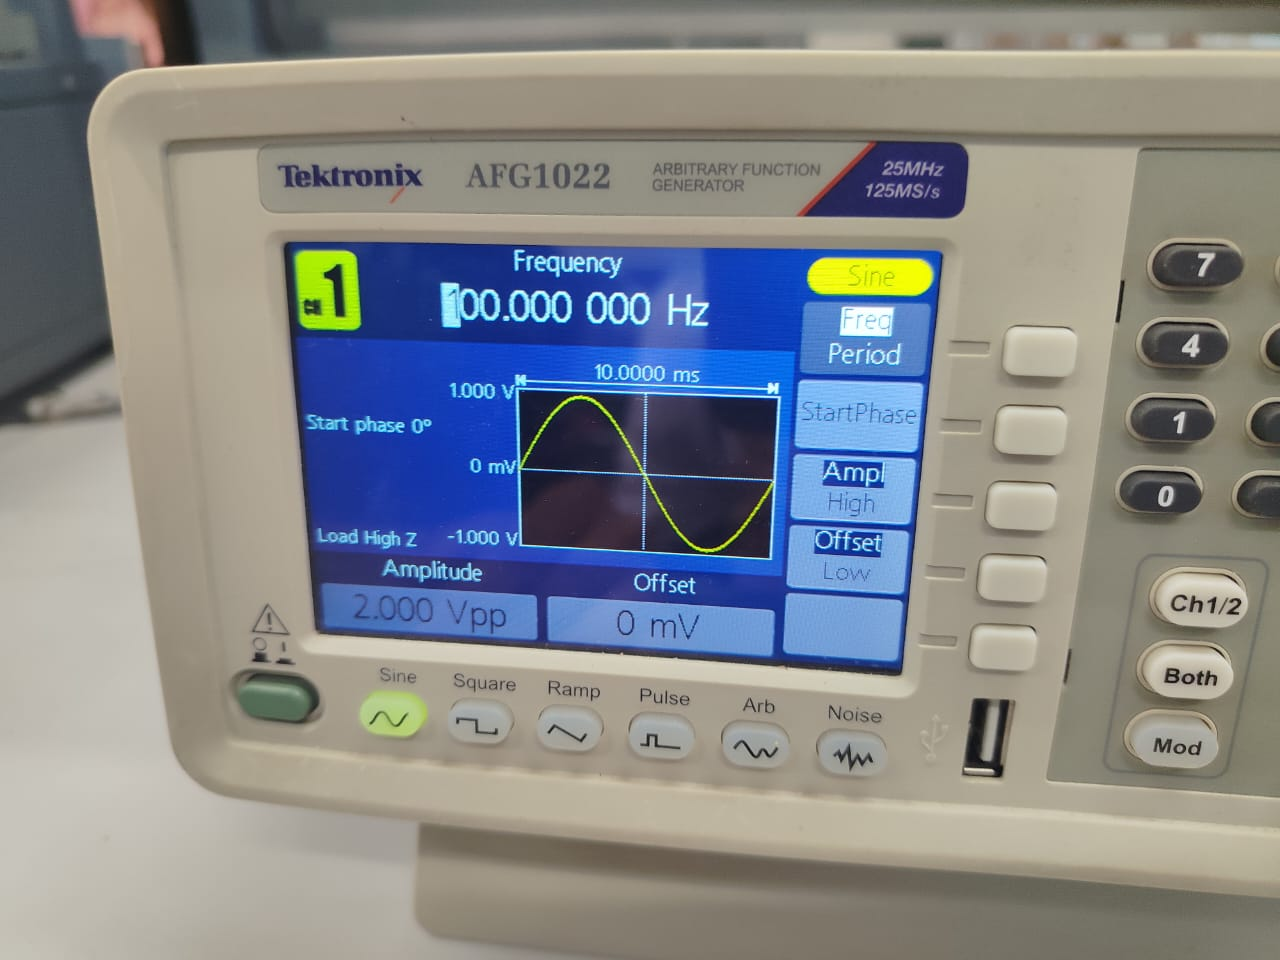
\includegraphics[width=0.45\textwidth]{figs/lowpassin4.jpeg}
    }
    \hfill
    \subfigure[Output]{
        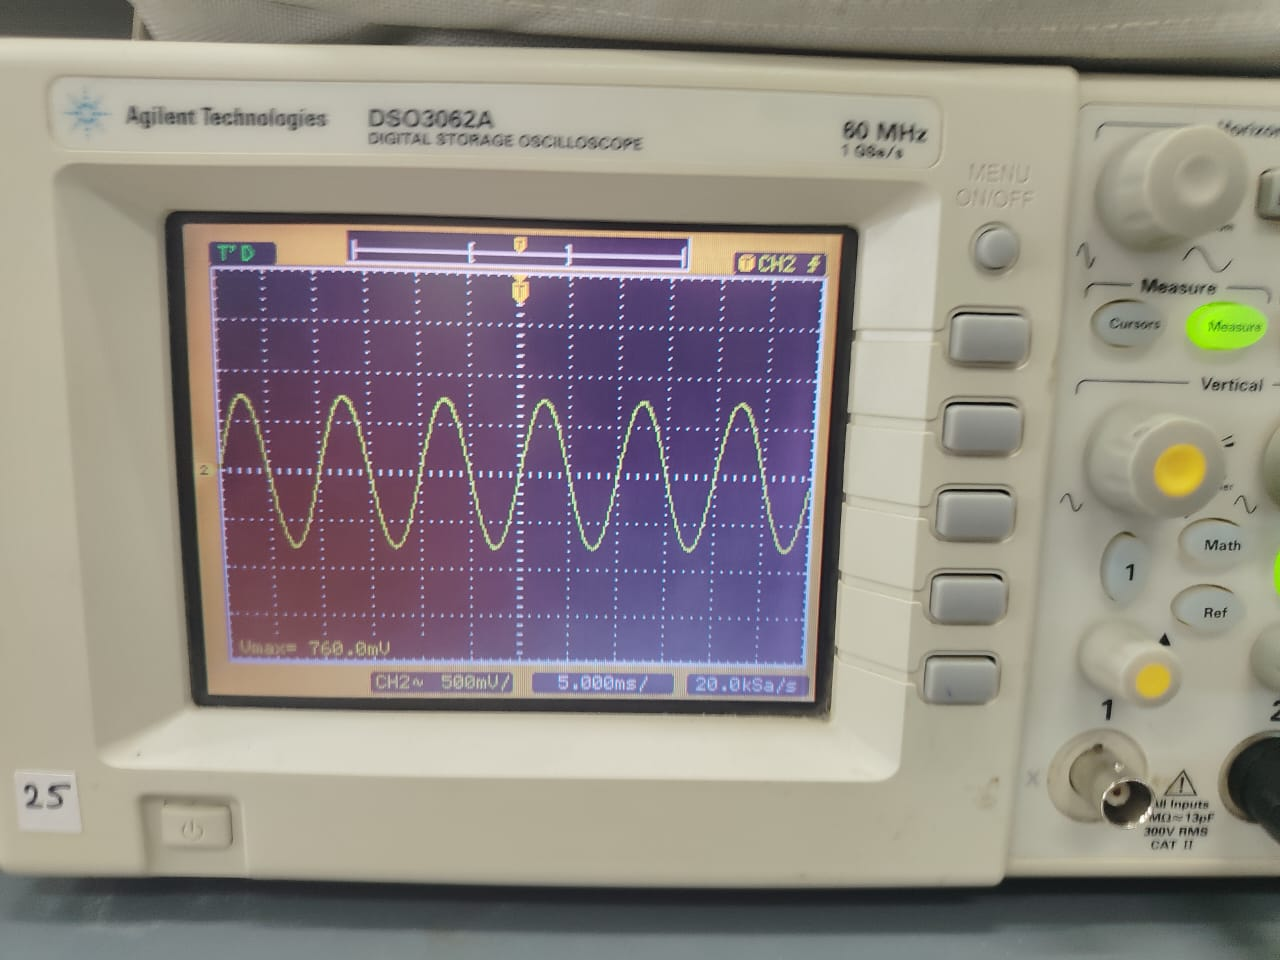
\includegraphics[width=0.45\textwidth]{figs/lowpassout4.jpeg}
    }
    \caption{Experimental results for low pass filter}
\end{figure}

% Add lowpass.png at the end of the low-pass filter section
\begin{figure}[H]
    \centering
    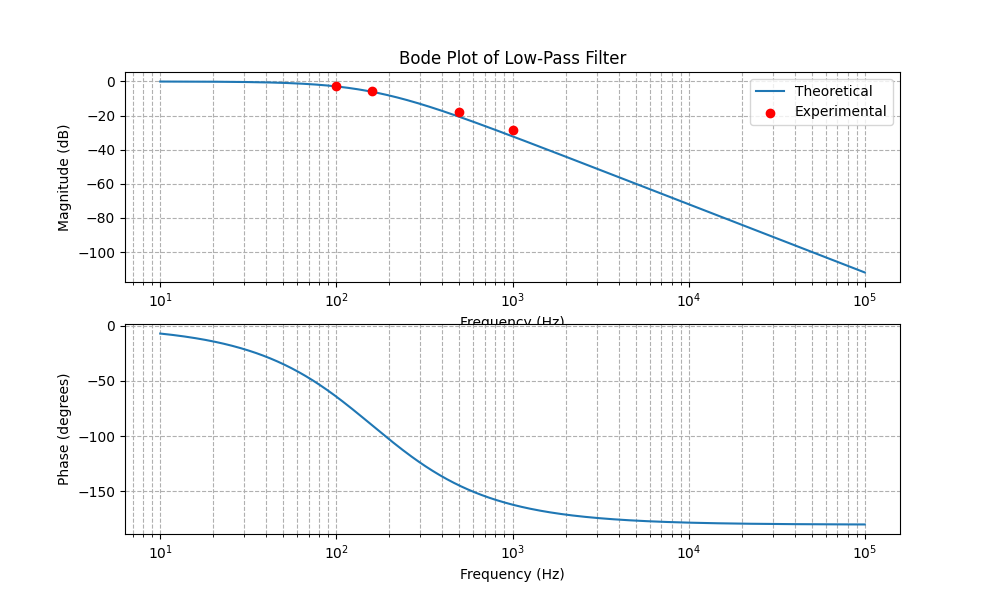
\includegraphics[width=0.8\textwidth]{figs/lowpass.png}
    \caption{Low Pass Filter Frequency Response}
\end{figure}

\subsection{Bandpass Sallen-Key Filter Design:}

% Two images side by side
\begin{figure}[H]
    \centering
    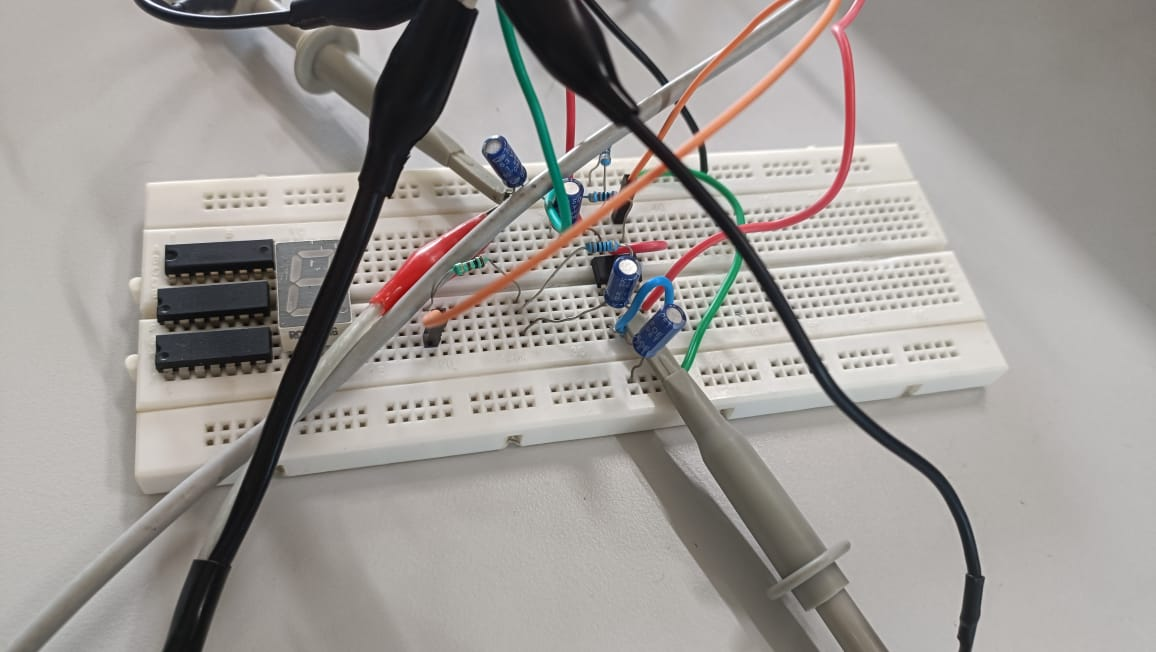
\includegraphics[width=0.8\textwidth]{figs/bandpasscircuit.jpeg}
    \caption{band Pass Sallen-Key Filter-Circuit design}
\end{figure}

\begin{itemize}
    \item The bandpass filter is constructed by cascading a high-pass filter and a low-pass filter.
    \item Components in the high-pass filter: R$_1$=R$_2$=1000$\Omega$ and C$_1$=C$_2$=1$\mu$F.
    \item Components in the low-pass filter: R$_1$=R$_2$=100$\Omega$ and C$_1$=C$_2$=1$\mu$F.
    \item The output of the high-pass filter is connected to the input of the low-pass filter.
    \item The overall transfer function of the bandpass filter is the product of the individual transfer functions of the high-pass and low-pass filters:
    \begin{align}
        H_{\text{BPF}}(s) = H_{\text{HPF}}(s) \cdot H_{\text{LPF}}(s)
    \end{align}
    where:
    \begin{align}
        H_{\text{HPF}}(s) = \frac{s^2}{s^2 + \frac{\omega_{c1}}{Q_1}s + \omega_{c1}^2}
    \end{align}
    \begin{align}
        H_{\text{LPF}}(s) = \frac{\omega_{c2}^2}{s^2 + \frac{\omega_{c2}}{Q_2}s + \omega_{c2}^2}
    \end{align}
    \item The cutoff frequencies for the high-pass and low-pass filters are:
    \begin{align}
        f_{c1} = 159.15 \text{ Hz} \quad (\text{High Pass}) \\
        f_{c2} = 1591.5 \text{ Hz} \quad (\text{Low Pass})
    \end{align}
    \item The bandpass filter allows frequencies between \( f_{c1} \) and \( f_{c2} \).
\end{itemize}

\textbf{Experimental Data}
\begin{table}[H]
    \centering
    \begin{tabular}{|c|c|c|c|c|}
        \hline
        Frequency (Hz) & Input Voltage (V) & Output Voltage (V) & Experimental Gain & Theoretical Gain\\
        \hline
        50 & 1.0 & 0.80 & -21.94 & -20.84 \\
        160 & 1.0 & 0.44 & -7.14 & -6.02 \\
        1000 & 1.0 & 0.90 & -3.56 & -3.8 \\
        1600 & 1.0 & 0. & -6.66 & -6.12 \\
        \hline
    \end{tabular}
    \caption{Comparison of Experimental and Theoretical Gain for Bandpass Filter}
    \label{tab:exp_data_bpf}
\end{table}
\begin{figure}[H]
    \centering
    \subfigure[Input]{
        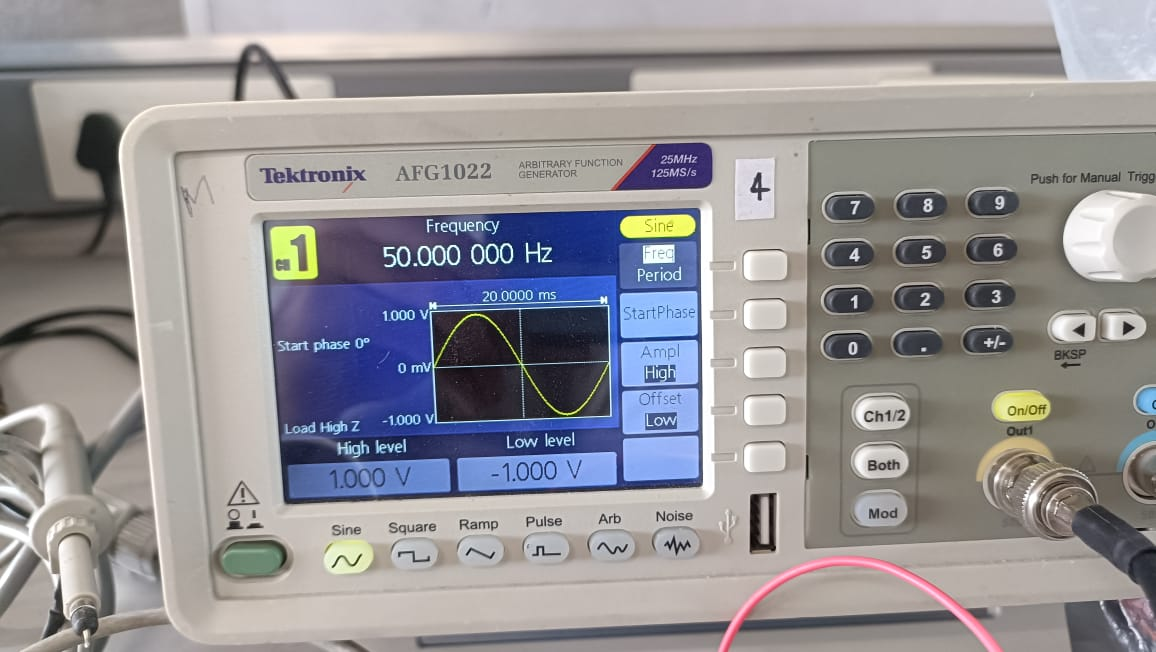
\includegraphics[width=0.45\textwidth]{figs/bandpassin1.jpeg}
    }
    \hfill
    \subfigure[Output]{
        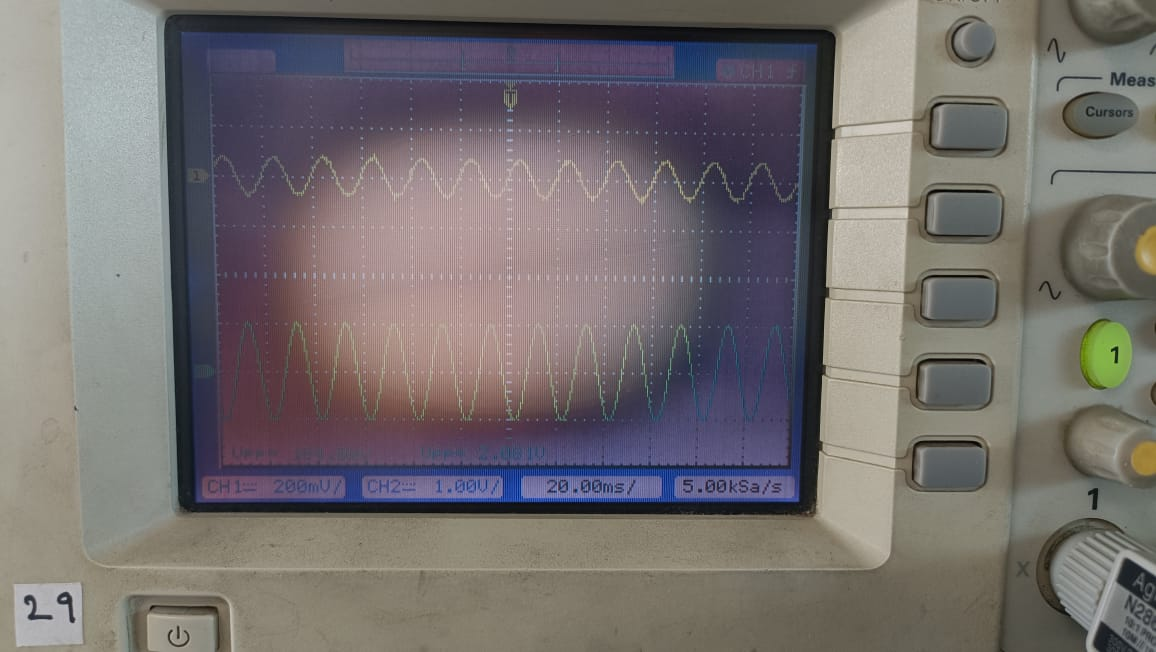
\includegraphics[width=0.45\textwidth]{figs/bandpassout1.jpeg}
    }
\end{figure}
\begin{figure}[H]
    \centering
    \subfigure[Input]{
        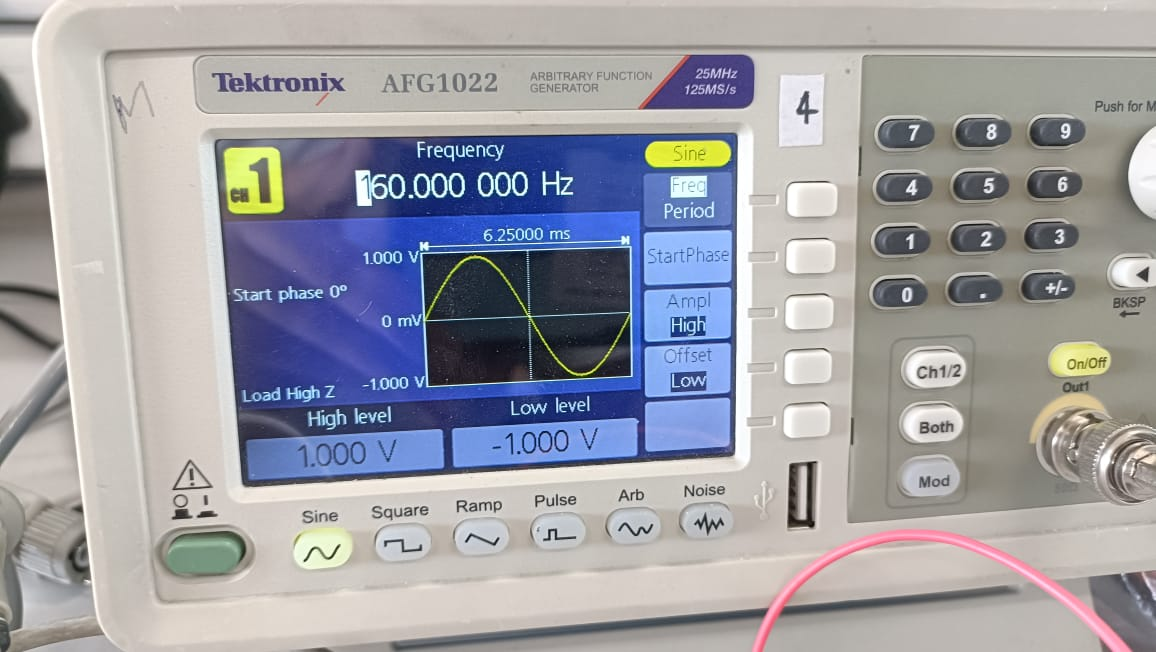
\includegraphics[width=0.45\textwidth]{figs/bandpassin2.jpeg}
    }
    \hfill
    \subfigure[Output]{
        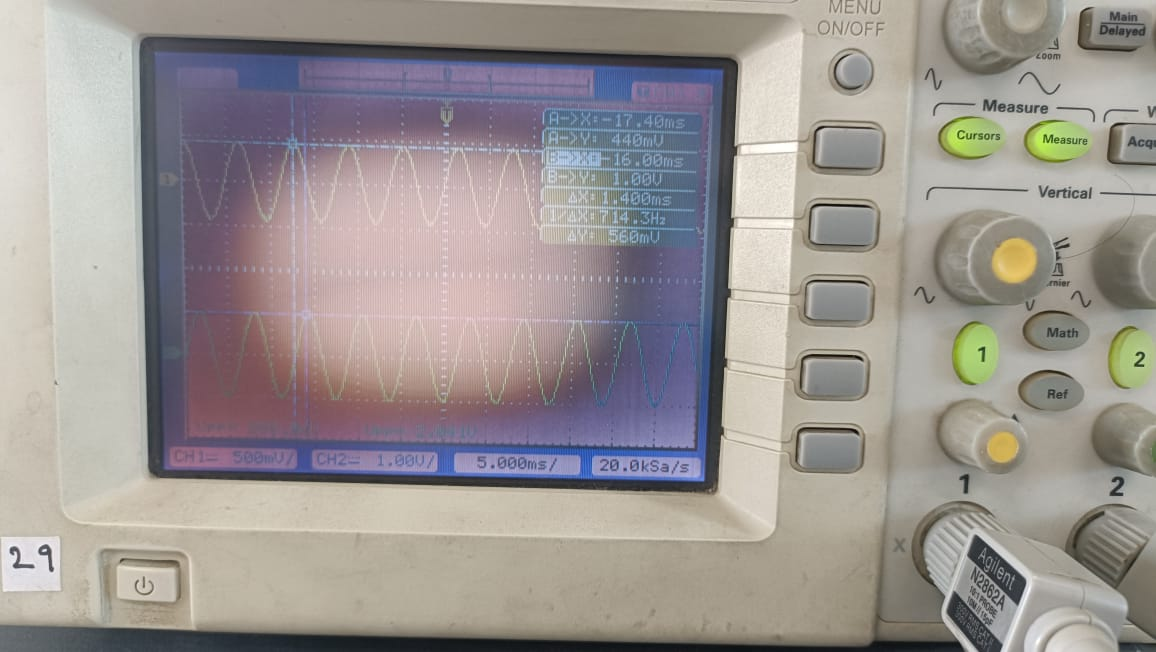
\includegraphics[width=0.45\textwidth]{figs/bandpassout2.jpeg}
    }
\end{figure}
\begin{figure}[H]
    \centering
    \subfigure[Input]{
        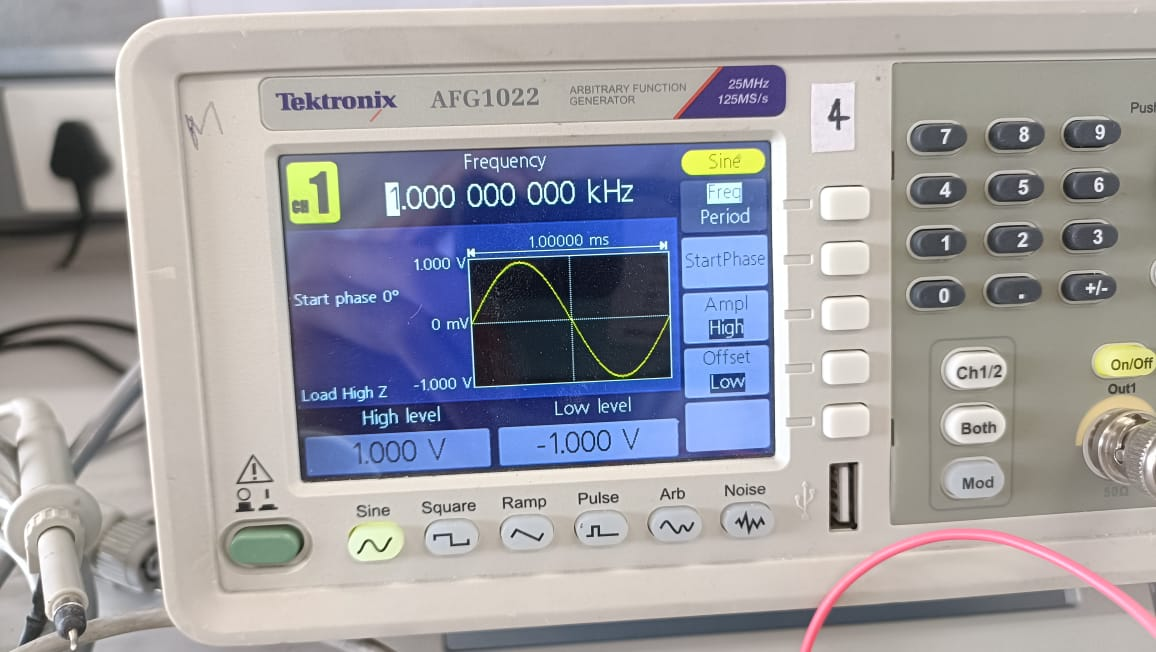
\includegraphics[width=0.45\textwidth]{figs/bandpassin3.jpeg}
    }
    \hfill
    \subfigure[Output]{
        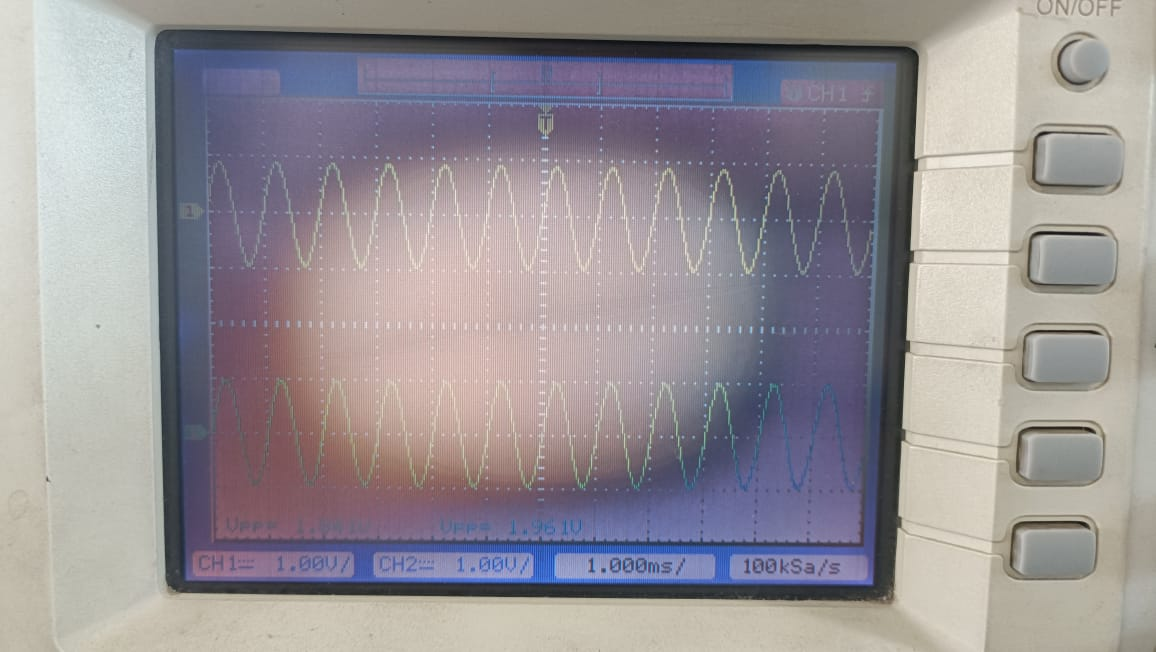
\includegraphics[width=0.45\textwidth]{figs/bandpassout3.jpeg}
    }
\end{figure}
\begin{figure}[H]
    \centering
    \subfigure[Input]{
        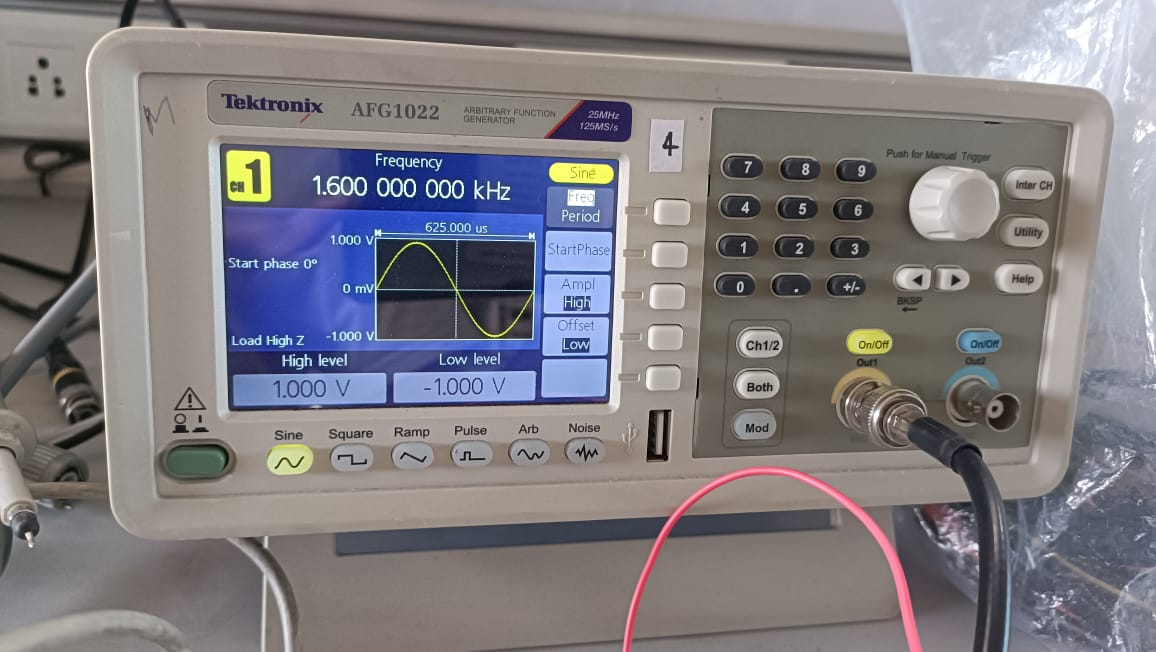
\includegraphics[width=0.45\textwidth]{figs/bandpassin4.jpeg}
    }
    \hfill
    \subfigure[Output]{
        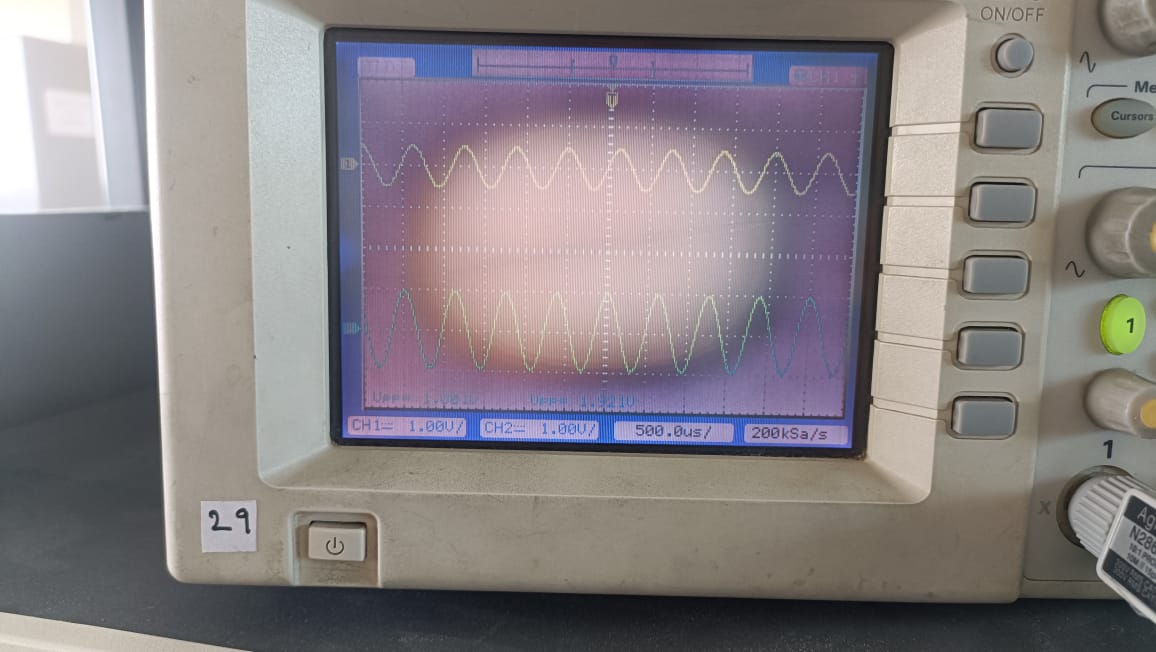
\includegraphics[width=0.45\textwidth]{figs/bandpassout4.jpeg}
    }
    \caption{Experimental results for bandpass filter}
\end{figure}

% Add bandpass.png at the end of the bandpass filter section
\begin{figure}[H]
    \centering
    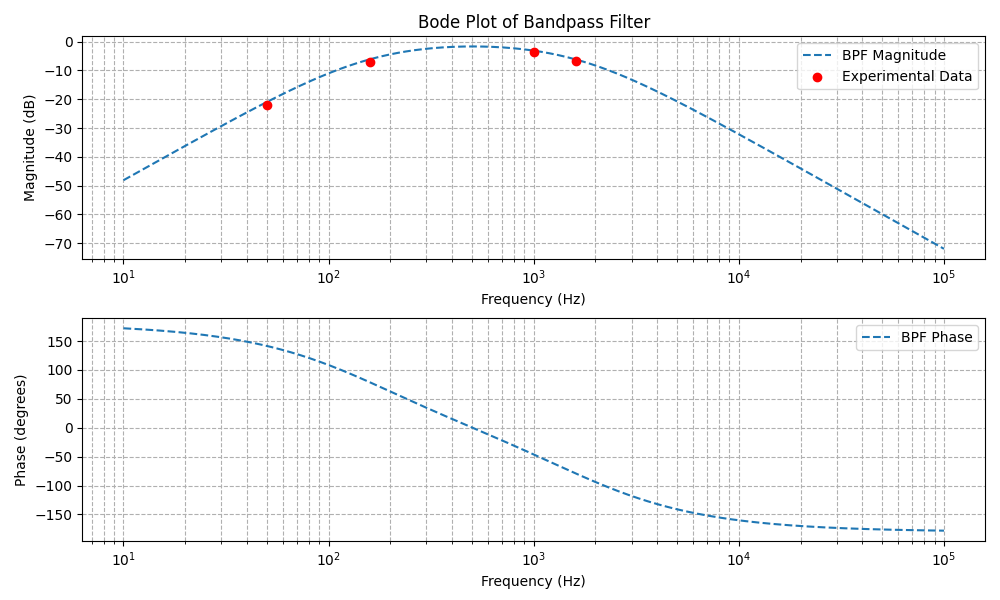
\includegraphics[width=0.8\textwidth]{figs/bandpass.png}
    \caption{Bandpass Filter Frequency Response}
\end{figure}
\section{Conclusion}
\begin{itemize}
    \item From the above observation we can say that cascading the low pass and high pass filter provides a good stability and response
\end{itemize}
For codes refer \href{https://github.com/ArnavYadnopavit/ElectricalLabEE1200/tree/main/Labreport6/codes}{this link}
\end{document}
